\documentclass[tikz,border=8pt]{standalone}
% Shared look for every TikZ diagram. Load with \input{../../tools/tikz-style.tex}
\usepackage[T1]{fontenc}
\usepackage{lmodern}
\renewcommand{\sfdefault}{lmr}  % diagrams use the same serif as the text
\usetikzlibrary{arrows.meta, positioning, shapes.geometric, calc, fit, backgrounds}
\definecolor{cblue}{HTML}{4C78A8}
\definecolor{corange}{HTML}{F58518}
\definecolor{cgreen}{HTML}{54A24B}
\definecolor{cred}{HTML}{E45756}
\definecolor{cpurple}{HTML}{B279A2}
\definecolor{cgrey}{HTML}{6B6B6B}
\tikzset{
  every picture/.style={font=\sffamily, line width=1.2pt},
  box/.style={draw=#1, fill=#1!12, rounded corners=4pt, align=center, inner sep=7pt, minimum height=1.1cm},
  box/.default=cgrey,
  arrow/.style={-{Stealth[length=3mm]}, draw=cgrey, line width=1.4pt},
  title/.style={font=\sffamily\bfseries\Large},
  note/.style={font=\sffamily\small, text=cgrey, align=center},
}
\AtBeginDocument{\hyphenpenalty=10000 \exhyphenpenalty=10000}

\begin{document}
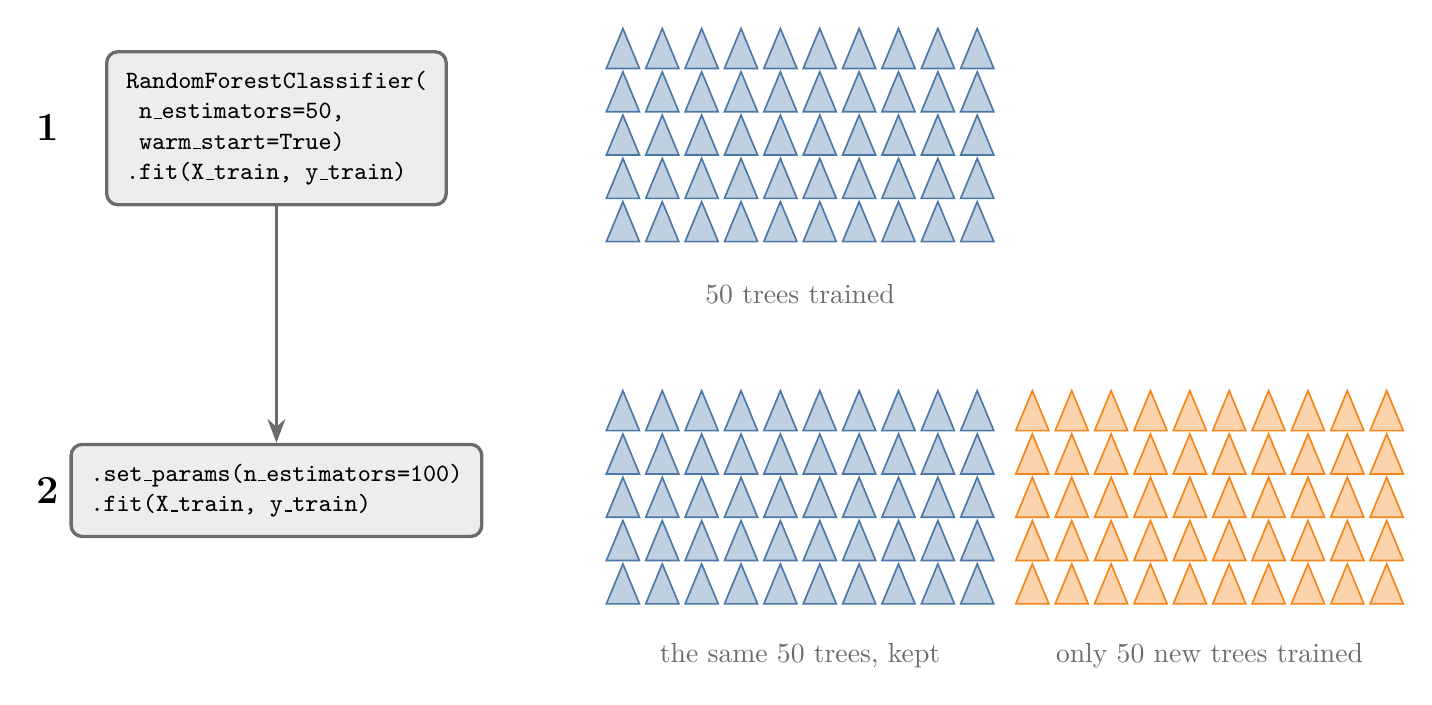
\begin{tikzpicture}[t/.style={draw=#1, fill=#1!35, isosceles triangle, shape border rotate=90, minimum width=0.42cm,
  minimum height=0.5cm, inner sep=0pt, line width=0.6pt}]
  % step 1
  \node[box=cgrey, font=\ttfamily\small, align=left] (a) at (0,0) {RandomForestClassifier(\\ \ n\_estimators=50,\\ \ warm\_start=True)\\.fit(X\_train, y\_train)};
  \foreach \i in {0,...,49} \node[t=cblue] at ({4.4+mod(\i,10)*0.5},{0.9-floor(\i/10)*0.55}) {};
  \node[note, font=\sffamily\normalsize] at (6.65,-2.1) {50 trees trained};
  % step 2
  \node[box=cgrey, font=\ttfamily\small, align=left] (b) at (0,-4.6) {.set\_params(n\_estimators=100)\\.fit(X\_train, y\_train)};
  \foreach \i in {0,...,49} \node[t=cblue] at ({4.4+mod(\i,10)*0.5},{-3.7-floor(\i/10)*0.55}) {};
  \foreach \i in {0,...,49} \node[t=corange] at ({9.6+mod(\i,10)*0.5},{-3.7-floor(\i/10)*0.55}) {};
  \node[note, font=\sffamily\normalsize] at (6.65,-6.7) {the same 50 trees, kept};
  \node[note, font=\sffamily\normalsize] at (11.85,-6.7) {only 50 new trees trained};
  \draw[arrow] (a.south) -- (b.north);
  \node[title] at (-2.9,0) {1}; \node[title] at (-2.9,-4.6) {2};
\end{tikzpicture}
\end{document}
